\documentclass{report}
\usepackage[utf8]{inputenc}

%----- Configuración del estilo del documento------%
\usepackage{epsfig,graphicx}
\usepackage[left=2.5cm,right=2.5cm,top=1.8cm,bottom=2.3cm]{geometry}
%------ Paquetes matematicos --------%
\usepackage{amsmath}
\usepackage{amssymb}
\usepackage{amsthm}
\usepackage{amsmath}
\usepackage{tabularx}
\usepackage{fancyhdr}
\usepackage{lastpage}
\usepackage{verbatim}
\usepackage[shortlabels]{enumitem}
\usepackage{venndiagram}
\usetikzlibrary{shapes.geometric}
\usepackage{cancel}
\usepackage{hyperref}
\usepackage[T1]{fontenc}
\usepackage[spanish,es-nodecimaldot,es-tabla]{babel}
\usepackage{csquotes}
\usepackage{graphicx}
\usepackage{tocloft}
\graphicspath{{./figs/}}
\usepackage{setspace}
\usepackage{xcolor}

%----- Configuración de las tablas ------%
\usepackage{array}
\usepackage{colortbl}
\usepackage{float} % Paquete necesario para usar [H]

%----- Configuración de la bibliografía ------%
\usepackage[backend=biber]{biblatex}
\addbibresource{resources/referencias/referencias.bib}


\begin{document}
	\begin{titlepage}
	\thispagestyle{empty}
	\begin{minipage}[c][0.17\textheight][c]{0.25\textwidth}
		\begin{center}
			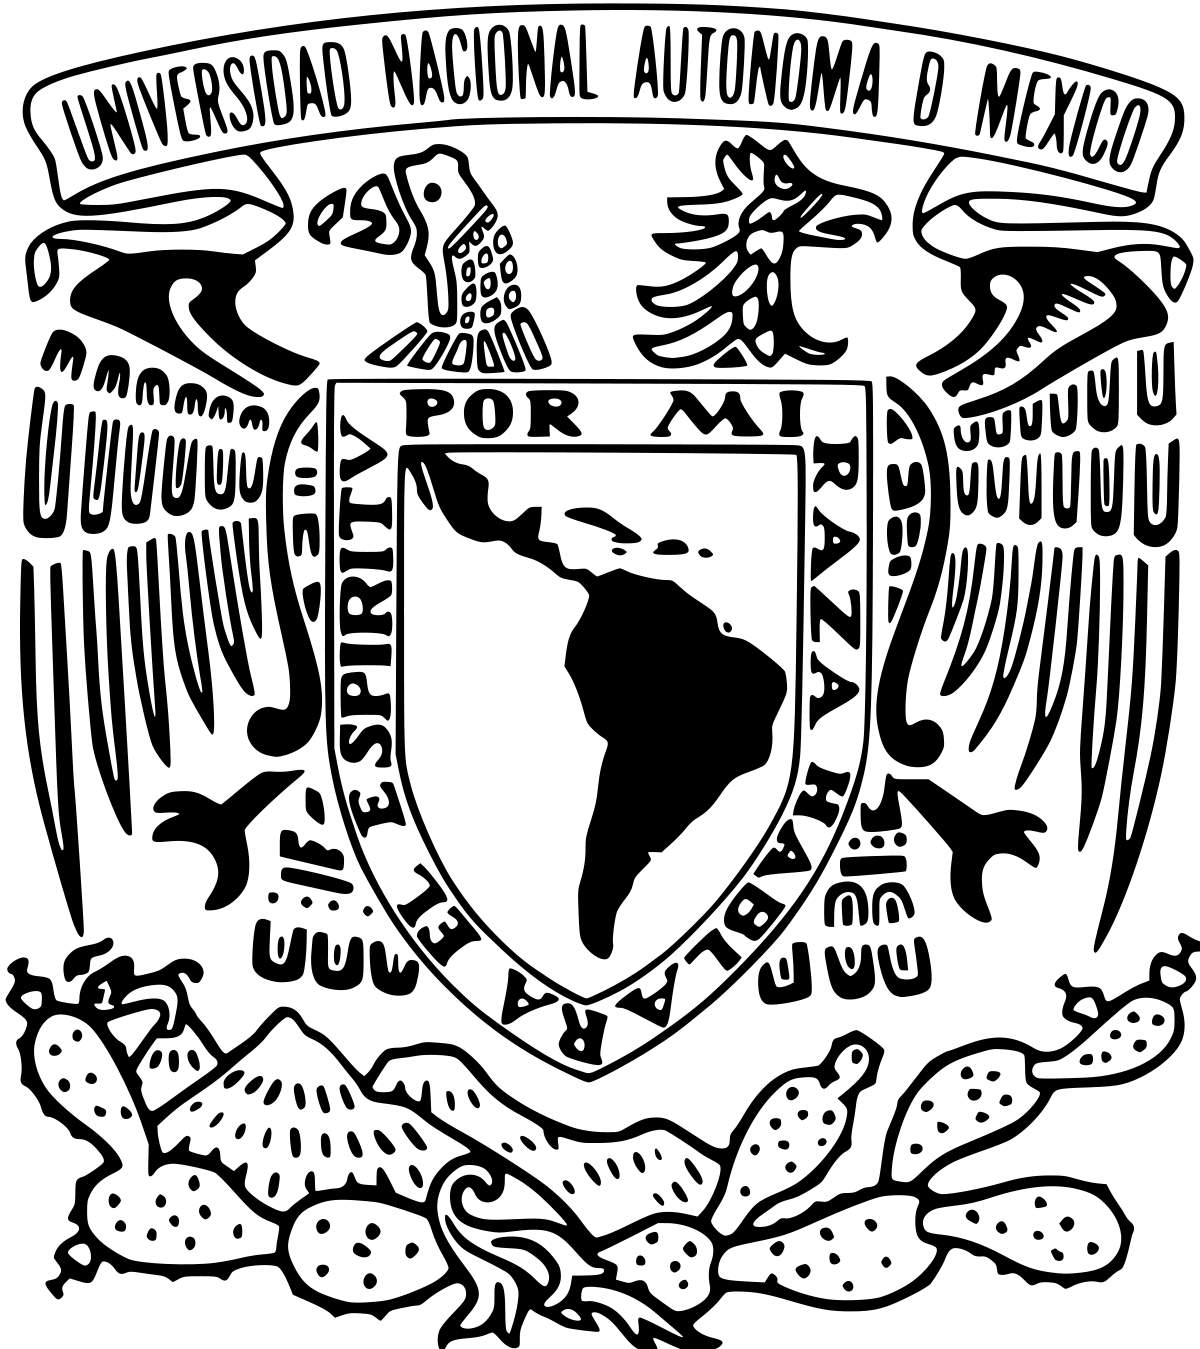
\includegraphics[width=3.5cm, height=3.5cm]{resources/Logo_UNAM.png}
		\end{center}
	\end{minipage}
	\begin{minipage}[c][0.195\textheight][t]{0.75\textwidth}
		\begin{center}
			\vspace{0.3cm}
			\textsc{\large Universidad Nacional Aut\'onoma de M\'exico}\\[0.5cm]
			\vspace{0.3cm}
			\hrule height2.5pt
			\vspace{.2cm}
			\hrule height1pt
			\vspace{.8cm}
			\textsc{Facultad de Ciencias}\\[0.5cm] %
		\end{center}
	\end{minipage}
	
	\begin{minipage}[c][0.81\textheight][t]{0.25\textwidth}
		\vspace*{5mm}
		\begin{center}
			\hskip2.0mm
			\vrule width1pt height13cm 
			\vspace{5mm}
			\hskip2pt
			\vrule width2.5pt height13cm
			\hskip2mm
			\vrule width1pt height13cm \\
			\vspace{5mm}
			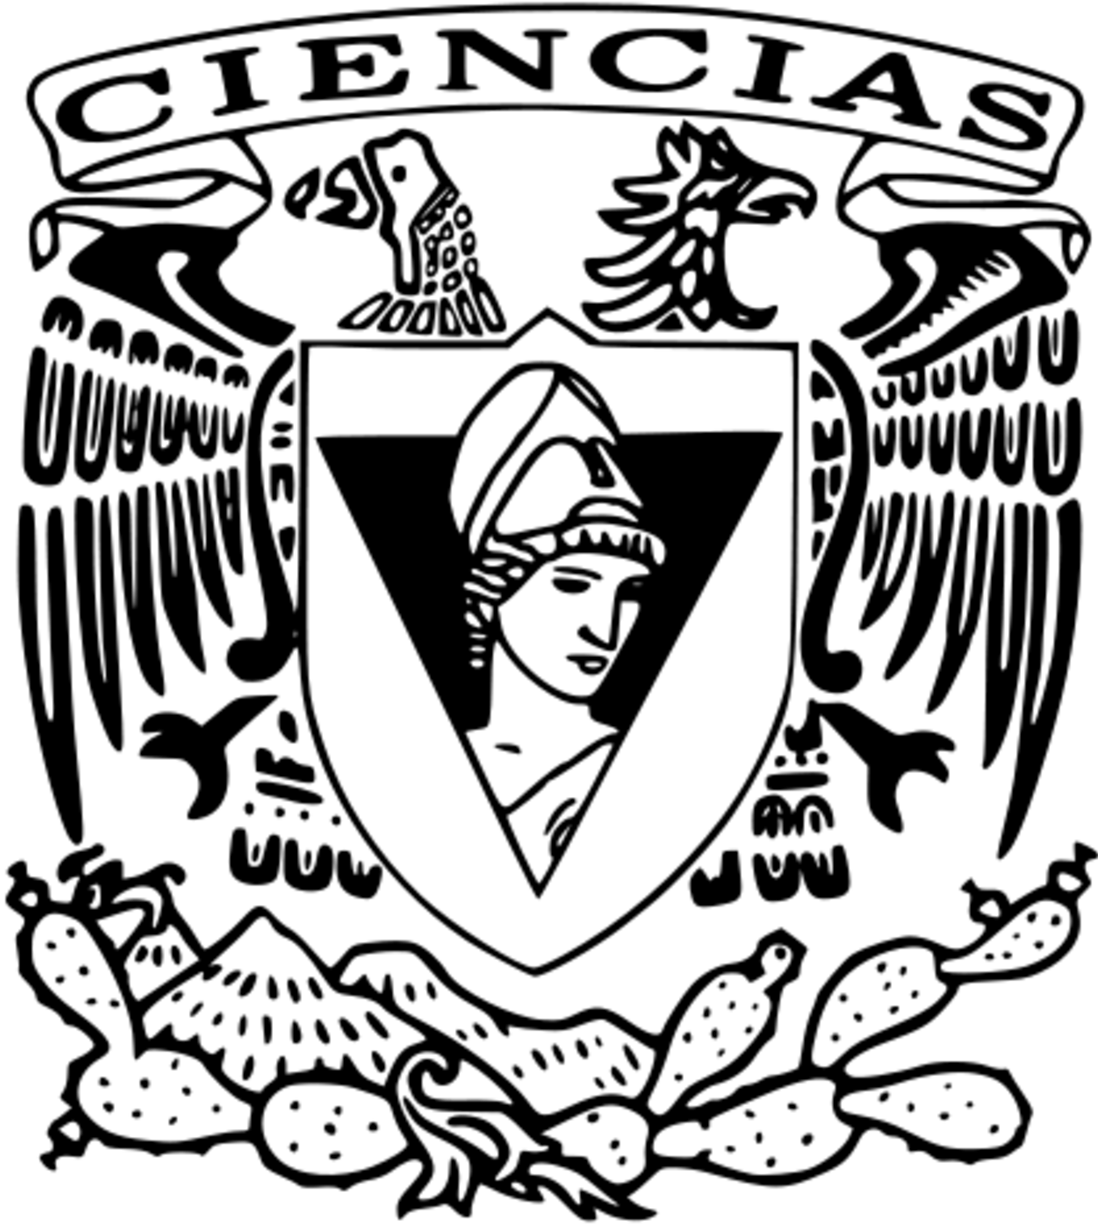
\includegraphics[height=4.0cm]{resources/Logo_FC.png}
		\end{center}
	\end{minipage}
	\begin{minipage}[c][0.81\textheight][t]{0.75\textwidth}
		\begin{center}
			\vspace{1cm}
			
			{\large\scshape Fundamentos de Bases de Datos - 7094}\\[.2in]
			
			\vspace{2cm}            
			
			\textsc{\LARGE \textbf{T}\hspace{1cm}\textbf{A}\hspace{1cm}\textbf{R}\hspace{1cm}\textbf{E}\hspace{1cm}\textbf{A}\hspace{1cm}\hspace{1cm}\textbf{4}}\\[2cm]
			\textsc{\Large{Equipo:}\normalsize \\
                \vspace{.3cm}
				\textbf{Del Monte Ortega Maryam Michelle - 320083527 \\
                \vspace{.2cm}
				\href{https://github.com/JuanSosaCiencias}{\textcolor{blue}{Sosa Romo Juan Mario - 320051926}} \\
                \vspace{.2cm}
				Castillo Hernández Antonio - 320017438 \\
                \vspace{.2cm}
                Erik Eduardo Gómez López - 320258211 \\
                \vspace{.2cm}
                Julio César Islas Espino - 320340594}}\\[0.5cm]     
			
			\textsc{{Fecha de entrega: \\ \textbf{10 de Octubre de 2024}}}\\[0.5cm]        
			
			\textsc{{Profesor: \\ \textbf{M. en I. Gerardo Avilés Rosas}}}\\[0.5cm]  
			
			\textsc{Ayudantes: \\ \textbf{Luis Enrique García Gómez \\ Kevin Jair Torres Valencia \\ Ricardo Badillo Macías \\ Rocío Aylin Huerta González
			} }
			
			
			\vspace{0.5cm}
		\end{center}
	\end{minipage}
\end{titlepage}

	
	\begin{center}
		\section*{\LARGE{Tarea 3}}
	\end{center}

    % Preguntas  
    \begin{center}
        \LARGE{\textbf{Preguntas de repaso}}\vspace{.3cm}
    \end{center}
    \normalsize
    \begin{enumerate}%[label=\alph*.]
        \item \begin{center}
    \textbf{Menciona 5 diferencias sentre almacenar la informacion utilizando un sistema de archivos o almacenarla utilizando una BDD.}
\end{center}

\begin{enumerate}
    \item \textbf{Estructura de Datos:} Los sistemas de archivos son simples colecciones de archivos sin relación entre ellos, mientras que             las bases de datos organizan los datos de manera estructurada y con relaciones lógicas.
    \item \textbf{Redundancia:} La redundancia de datos es alta en los sistemas de archivos, ya que los mismos datos pueden aparecer en                 múltiples lugares. En las bases de datos, la redundancia se minimiza mediante normalización.
    \item \textbf{Consistencia de Datos:} Los sistemas de archivos tienen problemas de inconsistencia cuando los datos se modifican en                 varios archivos. En las bases de datos, las actualizaciones se reflejan de manera consistente en todas las instancias de los datos.
    \item \textbf{Seguridad:} Los sistemas de archivos suelen ofrecer menos seguridad, mientras que las bases de datos incluyen medidas de             seguridad avanzadas como control de acceso y encriptación. 
    \item \textbf{Copia de Seguridad y recuperación:} Los sistemas de archivos no cuentan con mecanismos automatizados de respaldo y                     recuperación, mientras que las bases de datos generalmente incluyen estas funciones para proteger la información.\\
\end{enumerate}
\cite{guru99, sooluciona}

\vspace{.5cm}



        \item \textbf{¿Qué ventajas y desventajas encuentras al trabajar con un Sistema de Bases de Datos
considerando que se planea implantar este sistema en una empresa de telemarketing?} \\

En primera instancia tenemos que reconocer que el telemarketing es una técnica publicitaria que es utilizada por las empresas para contactar con potenciales clientes y hablarles acerca de sus productos o servicios . \\

Hay muchas empresas a lo largo del mundo que hacen de esta estrategia su principal manera de operar, catalogándose en mayor o menor medida como empresas de telemarketing y si bien cada empresa decide como gestionar sus recursos para así poder llegar a su publico objetivo, el telemarketing cuenta con una serie de ventajas y desventajas enumeradas de la siguiente manera las cuales pueden hacer que una empresa se decante por este sistema o no: \\


\begin{table}[h!]
    \centering
    \begin{tabular}{|p{6cm}||p{6cm}|}
        \hline
        \textcolor{blue}{\textbf{Ventajas}} & \textcolor{Red}{\textbf{Desventajas}} \\ \hline 
        Se tiene un trato mas directo con los potenciales clientes & Si se utiliza de manera inadecuada puede afectar negativamente a la reputación de la empresa \\ \hline
        Permite entrar en contacto con un gran número de clientes en poco tiempo & En algunos países existen ciertas restricciones para esta clase de técnicas \\ \hline 
        Permite ofrecer una gran cantidad de información sobre el producto o servicio en cuestión  & Requiere una inversión en formar a los agentes y que estos sigan las buenas practicas de la empresa \\ \hline
        Se puede llamar a cualquier parte del mundo, lo cual asegura que nuestra empresa pueda darse a conocer en otras fronteras & La tasa de conversión es baja\\ \hline
    \end{tabular}
    \caption{Ventajas y desventajas de un Sistema de Telemarketing \cite{boada_cyberclick_2023}} 
\end{table}

Así mismo el telemarketing puede utilizarse de distintas maneras y estas varían de acuerdo a la campaña y objetivos de la empresa. Pero volviendo al punto principal de la pregunta, algunas de las posibles ventajas y desventajas de implemmentar un sistema de base de datos en alguna empresa de telemarketing podrian ser las siguientes:\\


\begin{table}[h!]
    \centering
    \begin{tabular}{|p{6cm}||p{6cm}|}
        \hline
        \textcolor{green}{\textbf{Ventajas}} & \textcolor{purple}{\textbf{Desventajas}} \\ \hline
        Organización y gestión eficiente de datos & Altos costos de implementación y mantenimiento continuo. \\ \hline
        Generación de análisis detallados e historial de datos. & Trabajo extra para integración con sistemas existentes y necesidad de capacitación del personal. \\ \hline
         Automatiza las tareas repetitivas y hay una reducción de errores manuales. & Riesgo de interrupciones por fallos del sistema y necesidad de ajustes por actualizaciones. \\ \hline
        Tiene la capacidad para manejar más datos y mas personalización según necesidades específicas. &  Riesgos de seguridad y necesidad de cumplir con normativas de privacidad. \\ \hline
        Existe un control de acceso a datos sensibles y así como también un respaldo de datos. & Existen riesgos por parte de entradas de datos incorrectos y problemas de duplicados. \\ \hline
    \end{tabular}
    \caption{Ventajas y desventajas de un Sistema de BD en una empresa de telemarketing}
    \cite{adSalsa_2024}
\end{table}

        \item \textbf{Investiga que cuáles son las Reglas de Codd y explica con tus propias palabras cada una de ellas. Indica por qué
consideras que son importantes.}\vspace{.3cm}

    \end{enumerate}

    % Conversión de Modelo E/R a Modelo relacional  
    \begin{center}
        \LARGE{\textbf{Conversión de Modelo E/R a Modelo relacional  }}\vspace{.3cm}
    \end{center}
    \normalsize
    \begin{enumerate}[label=\alph*.]
        \item \textbf{Dos compañías con el nombre ‘Panaphonics’ podrían existir al mismo tiempo.}\vspace{.3cm}

\begin{quote}
    Voy a asumir que la relación \textbf{Proyecto} es donde se pondría el nombre de la compañía (que no se que tanto sentido tenga hacer esto para el departamento de RH de una empresa pero bueno). Vemos que en esta relación el único atributo que no se puede repetir es \textbf{NumProyecto} pues es la clave primaria. Por lo tanto, si se puede tener dos compañías con el nombre ‘Panaphonics’ al mismo tiempo. \vspace{.2cm}

    Si se quisiera que solo existiera una compañía con el nombre ‘Panaphonics’ al mismo tiempo, se podría definir el atributo \textbf{NombreCompañía} como clave primaria o una llave primaria compuesta con el atributo \textbf{NumProyecto}.
\end{quote}
\vspace{.3cm}
        \item \textbf{Del inciso a) toma el MR que obtuviste para la cardinalidad M : N. Asume que los atributos a1, b y ab1 son de tipo
entero, mientras que a2, a3 y b1 son de tipo cadena. Supón que la relación A tiene 4 tuplas con los siguientes valores
(2,’ww’,’a’), (4,’xx’,’b’), (6,’yy’,’c’), (8,’zz’,’d’) y la relación B tiene 5 tuplas identificadas por
los valores 17, 27, 37, 47, 57. Los incisos que se presentan a continuación, representan un conjunto de tuplas
a insertar (en ese orden) en la relación AB, indica cuál conjunto se puede insertar completamente en dicha relación.
Justifica tu respuesta en cada caso.}\vspace{.3cm}

\begin{enumerate}
    \item (8,’zz’,17,5); (6,’yy’,57,10); (4,’xx’,27,15); (2,’ww’,37,20); (4,’xx’,27,15)
    
    Podemos insertar (8,’zz’,17,5); (6,’yy’,57,10); (4,’xx’,27,15); (2,’ww’,37,20) y ya, insertar \textbf{otra vez} (4,’xx’,27,15) es innecesario ya que existiría más de una tupla con la misma llave.

    \item (17,’zz’,2,’m’); (27,’yy’,4,’n’); (37,’xx’,6,’o’); (47,’ww’,8,’p’); (57,’zz’,4,’q’)
    
    Ninguna se puede insertar ya que \textbf{ab1} es de tipo entero según las especificaciones y para este conjunto de tuplas, en todas se representa a \textbf{ab1} como cadena o caracter. 

    \item (2,’a’,17,23); (4,’b’,27,24); (6,’c’,37,25); (8,’d’,47,26); (2,’a’,57,27)
    
    Todas se pueden insertar, ya que los tipos de datos están correctos y no hay tuplas duplicadas ya que todas tienen más de un atributo distinto. 

    \item (2,’ww’,57,’a’); (4,’xx’,37,’b’); (6,’yy’,17,’c’); (8,’zz’,37,’d’); (4,’xx’,47,’a’)
    
    Nuevamente no podemos insertar ninguna ya que \textbf{ab1} es de tipo entero y se le pasan cadenas. 
\end{enumerate}

\vspace{.5cm}

    \end{enumerate}

    % Modelo relacional e inserción de tuplas. 
    \begin{center}
        \LARGE{\textbf{Modelo relacional e inserción de tuplas.}}\vspace{.3cm}
    \end{center}
    \normalsize
    \textbf{Atletas que hayan participado en más de 1 disciplina.}\vspace{.3cm}
    \begin{enumerate}[label=\alph*.]
        \item \textbf{Dos compañías con el nombre ‘Panaphonics’ podrían existir al mismo tiempo.}\vspace{.3cm}

\begin{quote}
    Voy a asumir que la relación \textbf{Proyecto} es donde se pondría el nombre de la compañía (que no se que tanto sentido tenga hacer esto para el departamento de RH de una empresa pero bueno). Vemos que en esta relación el único atributo que no se puede repetir es \textbf{NumProyecto} pues es la clave primaria. Por lo tanto, si se puede tener dos compañías con el nombre ‘Panaphonics’ al mismo tiempo. \vspace{.2cm}

    Si se quisiera que solo existiera una compañía con el nombre ‘Panaphonics’ al mismo tiempo, se podría definir el atributo \textbf{NombreCompañía} como clave primaria o una llave primaria compuesta con el atributo \textbf{NumProyecto}.
\end{quote}
\vspace{.3cm}
        \item \textbf{Del inciso a) toma el MR que obtuviste para la cardinalidad M : N. Asume que los atributos a1, b y ab1 son de tipo
entero, mientras que a2, a3 y b1 son de tipo cadena. Supón que la relación A tiene 4 tuplas con los siguientes valores
(2,’ww’,’a’), (4,’xx’,’b’), (6,’yy’,’c’), (8,’zz’,’d’) y la relación B tiene 5 tuplas identificadas por
los valores 17, 27, 37, 47, 57. Los incisos que se presentan a continuación, representan un conjunto de tuplas
a insertar (en ese orden) en la relación AB, indica cuál conjunto se puede insertar completamente en dicha relación.
Justifica tu respuesta en cada caso.}\vspace{.3cm}

\begin{enumerate}
    \item (8,’zz’,17,5); (6,’yy’,57,10); (4,’xx’,27,15); (2,’ww’,37,20); (4,’xx’,27,15)
    
    Podemos insertar (8,’zz’,17,5); (6,’yy’,57,10); (4,’xx’,27,15); (2,’ww’,37,20) y ya, insertar \textbf{otra vez} (4,’xx’,27,15) es innecesario ya que existiría más de una tupla con la misma llave.

    \item (17,’zz’,2,’m’); (27,’yy’,4,’n’); (37,’xx’,6,’o’); (47,’ww’,8,’p’); (57,’zz’,4,’q’)
    
    Ninguna se puede insertar ya que \textbf{ab1} es de tipo entero según las especificaciones y para este conjunto de tuplas, en todas se representa a \textbf{ab1} como cadena o caracter. 

    \item (2,’a’,17,23); (4,’b’,27,24); (6,’c’,37,25); (8,’d’,47,26); (2,’a’,57,27)
    
    Todas se pueden insertar, ya que los tipos de datos están correctos y no hay tuplas duplicadas ya que todas tienen más de un atributo distinto. 

    \item (2,’ww’,57,’a’); (4,’xx’,37,’b’); (6,’yy’,17,’c’); (8,’zz’,37,’d’); (4,’xx’,47,’a’)
    
    Nuevamente no podemos insertar ninguna ya que \textbf{ab1} es de tipo entero y se le pasan cadenas. 
\end{enumerate}

\vspace{.5cm}

        \item \textbf{Del inciso a) toma como base el MR que obtuviste para la cardinalidad 1 : N. Los incisos que se presentan a
continuación representan un conjunto de tuplas a insertar (en ese orden) en la relación B, indica cuál conjunto se
puede insertar completamente en dicha relación. Justifica tu respuesta en cada caso.}\vspace{.3cm}

\begin{enumerate}
    \item (2,’f’,57,’zz’); (4,’g’,47,’yy’); (6,’h’,37,’xx’); (8,’i’,27,’ww’); (2,’j’,17,’yy’)
    \item (57,8,’zz’,’f’); (47,6,’yy’,’g’); (37,4,’xx’,’h’); (27,2,’ww’,’i’); (17,6,’yy’,’j’)
    \item (57,’f’,8,’zz’); (47,’g’,6,’yy’); (37,’h’,4,’xx’); (27,’i’,2,’ww’); (17,’j’,6,’yy’)
    \item (57,’f’,8,’a’); (47,’g’,6,’b’); (37,’h’,4,’c’); (27,’i’,2,’d’); (17,’j’,6,’c’)
\end{enumerate}

\vspace{.5cm}

Tomando como base el modelo relacional obtenido para la relación 1:N del inciso a), procederemos a analizar cada conjunto de tuplas para determinar cuál de ellos se puede insertar completamente en la relación \texttt{B}. \\

\begin{enumerate}
    \item \textbf{(2,’f’,57,’zz’); (4,’g’,47,’yy’); (6,’h’,37,’xx’); (8,’i’,27,’ww’); (2,’j’,17,’yy’)} \\
    
    En este caso, los valores de \texttt{b} (57, 47, 37, 27, 17) son todos únicos, por lo que no hay problemas con la clave primaria en \texttt{B}. Además, las combinaciones de \texttt{a1} y \texttt{a2} (\texttt{(2,'zz')}, \texttt{(4,'yy')}, \texttt{(6,'xx')}, \texttt{(8,'ww')}, \texttt{(2,'yy')}) no generan conflictos en términos de las claves foráneas. Si estas combinaciones existen en la tabla \texttt{A}, se pueden insertar sin problemas. \\
    
    $\therefore$ El conjunto de tuplas se puede insertar completamente. \\

    \item \textbf{(57,8,’zz’,’f’); (47,6,’yy’,’g’); (37,4,’xx’,’h’); (27,2,’ww’,’i’); (17,6,’yy’,’j’)} \\
    
    Los valores de \texttt{b} (57, 47, 37, 27, 17) son diferentes, por lo que no hay conflictos con la clave primaria en \texttt{B}. Las combinaciones de \texttt{a1} y \texttt{a2} (\texttt{(8,'zz')}, \texttt{(6,'yy')}, \texttt{(4,'xx')}, \texttt{(2,'ww')}, \texttt{(6,'yy')}) muestran una repetición de \texttt{(6,'yy')}, pero mientras esa combinación sea válida en \texttt{A}, no debería haber problemas para insertar las tuplas en \texttt{B}. \\

    $\therefore$ El conjunto de tuplas se puede insertar completamente.\\

    \item \textbf{(57,’f’,8,’zz’); (47,’g’,6,’yy’); (37,’h’,4,’xx’); (27,’i’,2,’ww’); (17,’j’,6,’yy’)} \\
    
    En este conjunto, los valores de \texttt{b} (57, 47, 37, 27, 17) son únicos, lo cual es correcto para la clave primaria de \texttt{B}. Las combinaciones de \texttt{a1} y \texttt{a2} (\texttt{(8,'zz')}, \texttt{(6,'yy')}, \texttt{(4,'xx')}, \texttt{(2,'ww')}, \texttt{(6,'yy')}) incluyen una duplicación de \texttt{(6,'yy')}, pero si esta combinación es válida en \texttt{A}, no habría problemas para que las tuplas se inserten en \texttt{B}. \\

    $\therefore$ Este conjunto de tuplas se puede insertar completamente.

    \item \textbf{(57,’f’,8,’a’); (47,’g’,6,’b’); (37,’h’,4,’c’); (27,’i’,2,’d’); (17,’j’,6,’c’)} \\
    
    Aquí los valores de \texttt{b} (57, 47, 37, 27, 17) siguen siendo únicos, por lo que no hay conflicto con la clave primaria en \texttt{B}. Sin embargo, la combinación de \texttt{a1} y \texttt{a2} \texttt{(6,'c')} aparece en dos tuplas, lo cual es un problema, ya que \texttt{a1} y \texttt{a2} forman parte de la clave primaria compuesta en \texttt{A}. Esta duplicación no es válida, lo que viola la integridad referencial y, por lo tanto, no es posible insertar todas las tuplas. \\

    $\therefore$ Este conjunto de tuplas no se puede insertar completamente.
\end{enumerate}

        \item \textbf{Considera el mismo escenario del inciso b para las relaciones A y B. Toma como base el Modelo Relacional que
obtuviste para la cardinalidad 1:1. Supón que tu modelo tiene participación parcial de ambos lados. Propón un
conjunto de 4 tuplas que se pueda insertar en ab y un conjunto que no se pueda insertar (también de 4 tuplas).
Justifica tu respuesta en cada caso.}\vspace{.3cm}
\subsubsection*{Conjunto de 4 tuplas que se pueden insertar en \( AB \)}

Supongamos que las tuplas presentes en \( A \) y \( B \) son las siguientes:

\begin{itemize}
    \item \( A: (2, \text{'ww'}, \text{'a'}), (4, \text{'xx'}, \text{'b'}), (6, \text{'yy'}, \text{'c'}), (8, \text{'zz'}, \text{'d'}) \)
    \item \( B: (17, \text{'e'}), (27, \text{'f'}), (37, \text{'g'}), (47, \text{'h'}) \)
\end{itemize}

Propuestas de tuplas para \( AB \):

\begin{enumerate}
    \item (2, \text{'ww'}, 17, 10)
    \item (4, \text{'xx'}, 27, 20)
    \item (6, \text{'yy'}, 37, 30)
    \item (8, \text{'zz'}, 47, 40)
\end{enumerate}


Estas tuplas se pueden insertar porque:

\begin{itemize}
    \item Cada \( (a1, a2) \) de \( AB \) corresponde a una combinación válida de claves primarias de \( A \).
    \item Cada \( b \) en \( AB \) coincide con una clave primaria en \( B \).
    \item Las combinaciones de \( (a1, a2) \) y \( b \) son únicas, respetando la restricción de 1:1, sin repetir la asociación entre \( A \) y \( B \).
\end{itemize}

\subsubsection*{Conjunto de 4 tuplas que no se pueden insertar en \( AB \)}

\begin{enumerate}
    \item (2, \text{'ww'}, 17, 10)
    \item (2, \text{'ww'}, 27, 20)
    \item (4, \text{'xx'}, 27, 30)
    \item (4, \text{'xx'}, 47, 40)
\end{enumerate}


Estas tuplas no se pueden insertar debido a que:

\begin{itemize}
    \item Las primeras dos tuplas intentan asociar la misma tupla de \( A \) (\( 2, \text{'ww'} \)) con diferentes tuplas de \( B \) (17 y 27), violando la restricción de 1:1.
    \item Las últimas dos tuplas intentan asociar la misma tupla de \( A \) (\( 4, \text{'xx'} \)) con diferentes tuplas de \( B \) (27 y 47), lo cual también infringe la relación 1:1.
    \item La relación 1:1 implica que una tupla de \( A \) solo puede estar asociada con una única tupla de \( B \) y viceversa, y estas tuplas propuestas intentan establecer múltiples asociaciones.
\end{itemize}

    \end{enumerate}

    % Modelo relacional y restricciones de integridad 
    \begin{center}
        \LARGE{\textbf{Modelo relacional y restricciones de integridad}}\vspace{.3cm}
    \end{center}
    \normalsize
    
Cómo modificarías el diagrama de la figura a) para representar las siguientes restricciones:\\
Un alumno no puede tomar clase en más de una materia con el mismo profesor. Una materia no puede ser
impartida por más de un profesor.

No es necesario realizar alguna modificación, pues la cardinalidad uno a uno que tiene el diagrama implica que un alumno no puede estar relacionado con el mismo profesor en más de una materia, y del mismo modo una materia no puede ser impartida por más de un profesor en la relación, por lo que el diagrama ya cumple con ambas restricciones.

    \begin{enumerate}[label=\alph*.]
        \item \textbf{Dos compañías con el nombre ‘Panaphonics’ podrían existir al mismo tiempo.}\vspace{.3cm}

\begin{quote}
    Voy a asumir que la relación \textbf{Proyecto} es donde se pondría el nombre de la compañía (que no se que tanto sentido tenga hacer esto para el departamento de RH de una empresa pero bueno). Vemos que en esta relación el único atributo que no se puede repetir es \textbf{NumProyecto} pues es la clave primaria. Por lo tanto, si se puede tener dos compañías con el nombre ‘Panaphonics’ al mismo tiempo. \vspace{.2cm}

    Si se quisiera que solo existiera una compañía con el nombre ‘Panaphonics’ al mismo tiempo, se podría definir el atributo \textbf{NombreCompañía} como clave primaria o una llave primaria compuesta con el atributo \textbf{NumProyecto}.
\end{quote}
\vspace{.3cm}
        \item \textbf{Del inciso a) toma el MR que obtuviste para la cardinalidad M : N. Asume que los atributos a1, b y ab1 son de tipo
entero, mientras que a2, a3 y b1 son de tipo cadena. Supón que la relación A tiene 4 tuplas con los siguientes valores
(2,’ww’,’a’), (4,’xx’,’b’), (6,’yy’,’c’), (8,’zz’,’d’) y la relación B tiene 5 tuplas identificadas por
los valores 17, 27, 37, 47, 57. Los incisos que se presentan a continuación, representan un conjunto de tuplas
a insertar (en ese orden) en la relación AB, indica cuál conjunto se puede insertar completamente en dicha relación.
Justifica tu respuesta en cada caso.}\vspace{.3cm}

\begin{enumerate}
    \item (8,’zz’,17,5); (6,’yy’,57,10); (4,’xx’,27,15); (2,’ww’,37,20); (4,’xx’,27,15)
    
    Podemos insertar (8,’zz’,17,5); (6,’yy’,57,10); (4,’xx’,27,15); (2,’ww’,37,20) y ya, insertar \textbf{otra vez} (4,’xx’,27,15) es innecesario ya que existiría más de una tupla con la misma llave.

    \item (17,’zz’,2,’m’); (27,’yy’,4,’n’); (37,’xx’,6,’o’); (47,’ww’,8,’p’); (57,’zz’,4,’q’)
    
    Ninguna se puede insertar ya que \textbf{ab1} es de tipo entero según las especificaciones y para este conjunto de tuplas, en todas se representa a \textbf{ab1} como cadena o caracter. 

    \item (2,’a’,17,23); (4,’b’,27,24); (6,’c’,37,25); (8,’d’,47,26); (2,’a’,57,27)
    
    Todas se pueden insertar, ya que los tipos de datos están correctos y no hay tuplas duplicadas ya que todas tienen más de un atributo distinto. 

    \item (2,’ww’,57,’a’); (4,’xx’,37,’b’); (6,’yy’,17,’c’); (8,’zz’,37,’d’); (4,’xx’,47,’a’)
    
    Nuevamente no podemos insertar ninguna ya que \textbf{ab1} es de tipo entero y se le pasan cadenas. 
\end{enumerate}

\vspace{.5cm}

        \item \textbf{Del inciso a) toma como base el MR que obtuviste para la cardinalidad 1 : N. Los incisos que se presentan a
continuación representan un conjunto de tuplas a insertar (en ese orden) en la relación B, indica cuál conjunto se
puede insertar completamente en dicha relación. Justifica tu respuesta en cada caso.}\vspace{.3cm}

\begin{enumerate}
    \item (2,’f’,57,’zz’); (4,’g’,47,’yy’); (6,’h’,37,’xx’); (8,’i’,27,’ww’); (2,’j’,17,’yy’)
    \item (57,8,’zz’,’f’); (47,6,’yy’,’g’); (37,4,’xx’,’h’); (27,2,’ww’,’i’); (17,6,’yy’,’j’)
    \item (57,’f’,8,’zz’); (47,’g’,6,’yy’); (37,’h’,4,’xx’); (27,’i’,2,’ww’); (17,’j’,6,’yy’)
    \item (57,’f’,8,’a’); (47,’g’,6,’b’); (37,’h’,4,’c’); (27,’i’,2,’d’); (17,’j’,6,’c’)
\end{enumerate}

\vspace{.5cm}

Tomando como base el modelo relacional obtenido para la relación 1:N del inciso a), procederemos a analizar cada conjunto de tuplas para determinar cuál de ellos se puede insertar completamente en la relación \texttt{B}. \\

\begin{enumerate}
    \item \textbf{(2,’f’,57,’zz’); (4,’g’,47,’yy’); (6,’h’,37,’xx’); (8,’i’,27,’ww’); (2,’j’,17,’yy’)} \\
    
    En este caso, los valores de \texttt{b} (57, 47, 37, 27, 17) son todos únicos, por lo que no hay problemas con la clave primaria en \texttt{B}. Además, las combinaciones de \texttt{a1} y \texttt{a2} (\texttt{(2,'zz')}, \texttt{(4,'yy')}, \texttt{(6,'xx')}, \texttt{(8,'ww')}, \texttt{(2,'yy')}) no generan conflictos en términos de las claves foráneas. Si estas combinaciones existen en la tabla \texttt{A}, se pueden insertar sin problemas. \\
    
    $\therefore$ El conjunto de tuplas se puede insertar completamente. \\

    \item \textbf{(57,8,’zz’,’f’); (47,6,’yy’,’g’); (37,4,’xx’,’h’); (27,2,’ww’,’i’); (17,6,’yy’,’j’)} \\
    
    Los valores de \texttt{b} (57, 47, 37, 27, 17) son diferentes, por lo que no hay conflictos con la clave primaria en \texttt{B}. Las combinaciones de \texttt{a1} y \texttt{a2} (\texttt{(8,'zz')}, \texttt{(6,'yy')}, \texttt{(4,'xx')}, \texttt{(2,'ww')}, \texttt{(6,'yy')}) muestran una repetición de \texttt{(6,'yy')}, pero mientras esa combinación sea válida en \texttt{A}, no debería haber problemas para insertar las tuplas en \texttt{B}. \\

    $\therefore$ El conjunto de tuplas se puede insertar completamente.\\

    \item \textbf{(57,’f’,8,’zz’); (47,’g’,6,’yy’); (37,’h’,4,’xx’); (27,’i’,2,’ww’); (17,’j’,6,’yy’)} \\
    
    En este conjunto, los valores de \texttt{b} (57, 47, 37, 27, 17) son únicos, lo cual es correcto para la clave primaria de \texttt{B}. Las combinaciones de \texttt{a1} y \texttt{a2} (\texttt{(8,'zz')}, \texttt{(6,'yy')}, \texttt{(4,'xx')}, \texttt{(2,'ww')}, \texttt{(6,'yy')}) incluyen una duplicación de \texttt{(6,'yy')}, pero si esta combinación es válida en \texttt{A}, no habría problemas para que las tuplas se inserten en \texttt{B}. \\

    $\therefore$ Este conjunto de tuplas se puede insertar completamente.

    \item \textbf{(57,’f’,8,’a’); (47,’g’,6,’b’); (37,’h’,4,’c’); (27,’i’,2,’d’); (17,’j’,6,’c’)} \\
    
    Aquí los valores de \texttt{b} (57, 47, 37, 27, 17) siguen siendo únicos, por lo que no hay conflicto con la clave primaria en \texttt{B}. Sin embargo, la combinación de \texttt{a1} y \texttt{a2} \texttt{(6,'c')} aparece en dos tuplas, lo cual es un problema, ya que \texttt{a1} y \texttt{a2} forman parte de la clave primaria compuesta en \texttt{A}. Esta duplicación no es válida, lo que viola la integridad referencial y, por lo tanto, no es posible insertar todas las tuplas. \\

    $\therefore$ Este conjunto de tuplas no se puede insertar completamente.
\end{enumerate}

        \item \textbf{Considera el mismo escenario del inciso b para las relaciones A y B. Toma como base el Modelo Relacional que
obtuviste para la cardinalidad 1:1. Supón que tu modelo tiene participación parcial de ambos lados. Propón un
conjunto de 4 tuplas que se pueda insertar en ab y un conjunto que no se pueda insertar (también de 4 tuplas).
Justifica tu respuesta en cada caso.}\vspace{.3cm}
\subsubsection*{Conjunto de 4 tuplas que se pueden insertar en \( AB \)}

Supongamos que las tuplas presentes en \( A \) y \( B \) son las siguientes:

\begin{itemize}
    \item \( A: (2, \text{'ww'}, \text{'a'}), (4, \text{'xx'}, \text{'b'}), (6, \text{'yy'}, \text{'c'}), (8, \text{'zz'}, \text{'d'}) \)
    \item \( B: (17, \text{'e'}), (27, \text{'f'}), (37, \text{'g'}), (47, \text{'h'}) \)
\end{itemize}

Propuestas de tuplas para \( AB \):

\begin{enumerate}
    \item (2, \text{'ww'}, 17, 10)
    \item (4, \text{'xx'}, 27, 20)
    \item (6, \text{'yy'}, 37, 30)
    \item (8, \text{'zz'}, 47, 40)
\end{enumerate}


Estas tuplas se pueden insertar porque:

\begin{itemize}
    \item Cada \( (a1, a2) \) de \( AB \) corresponde a una combinación válida de claves primarias de \( A \).
    \item Cada \( b \) en \( AB \) coincide con una clave primaria en \( B \).
    \item Las combinaciones de \( (a1, a2) \) y \( b \) son únicas, respetando la restricción de 1:1, sin repetir la asociación entre \( A \) y \( B \).
\end{itemize}

\subsubsection*{Conjunto de 4 tuplas que no se pueden insertar en \( AB \)}

\begin{enumerate}
    \item (2, \text{'ww'}, 17, 10)
    \item (2, \text{'ww'}, 27, 20)
    \item (4, \text{'xx'}, 27, 30)
    \item (4, \text{'xx'}, 47, 40)
\end{enumerate}


Estas tuplas no se pueden insertar debido a que:

\begin{itemize}
    \item Las primeras dos tuplas intentan asociar la misma tupla de \( A \) (\( 2, \text{'ww'} \)) con diferentes tuplas de \( B \) (17 y 27), violando la restricción de 1:1.
    \item Las últimas dos tuplas intentan asociar la misma tupla de \( A \) (\( 4, \text{'xx'} \)) con diferentes tuplas de \( B \) (27 y 47), lo cual también infringe la relación 1:1.
    \item La relación 1:1 implica que una tupla de \( A \) solo puede estar asociada con una única tupla de \( B \) y viceversa, y estas tuplas propuestas intentan establecer múltiples asociaciones.
\end{itemize}

        \item 
Explica el concepto de categorías (herencia múltiple) en el modelo E-R y proporciona dos ejemplos de la vida real en donde se aplique este concepto.

Las \textbf{categorías} (o herencia múltiple) en el modelo E-R permite que una entidad pueda heredar sus atributos a otras entidades, donde la entidad hija \textbf{(subtipo)}, hereda los atributos y relaciones de una o múltiples entidades padres \textbf{(supertipo)}. Esto significa que la entidad hija se relaciona con varias entidades padres, combinando sus características.

Ejemplos:
\begin{itemize}
    \item \textbf{Ejemplo 1:}
    \begin{itemize}
        \item \textbf{Supertipo: } Empleado y Consultor
        \item \textbf{Subtipo:} Empleado-Consultor
        
    \begin{itemize}
        \item La entidad \textbf{Empleado} contiene atributos como 'Número de empleado', 'Salario', 'Departamento'.
        \item La entidad \textbf{Consultor} tiene atributos como 'Número de proyecto', 'Tarifa por hora', 'Fecha de finalización'.
        \item La entidad \textbf{Empleado-Consultor} hereda atributos tanto de \textbf{Empleado} como de \textbf{Consultor}, y puede tener atributos adicionales como 'Horas dedicadas como consultor'. Esta entidad representa a un trabajador que es tanto un empleado fijo de una empresa como un consultor en proyectos específicos.
    \end{itemize}
    \end{itemize}

    \item \textbf{Ejemplo 2:}
    \begin{itemize}
         \item \textbf{Supertipo:} Persona
        \item \textbf{Subtipo:} Estudiante y Profesor
        
    \begin{itemize}
        \item La entidad \textbf{Persona} contiene atributos comunes como 'Nombre', 'Edad" y 'Dirección'.
        \item Las entidades hijas \textbf{Estudiante} y \textbf{Profesor} heredan esos atributos comunes, pero tienen atributos adicionales específicos:
        \begin{itemize}
            \item \textbf{Estudiante:} 'Número de matrícula', 'Carrera'.
            \item \textbf{Profesor:} 'Número de empleado', 'Departamento'.
        \end{itemize}
    \end{itemize}
    \end{itemize}
\end{itemize}

        \item \textbf{Se puede almacenar ‘Laramie Cigarettes’ sin necesidad de definir a un director}\vspace{.3cm}
Verdadero. La existencia de un proyecto en la tabla \texttt{Proyecto} no depende de la relación \texttt{Dirigir}, por lo que un proyecto puede ser almacenado sin que se defina un director.

        \item \textbf{Los empleados y/o directores deben vivir en la misma Ciudad que la Compañía para la que laboran/dirigen.}\vspace{.3cm} \\

Para que ePara que esta afirmación fuera verdadera, debería existir una relación entre la ciudad donde reside un empleado o director y la ubicación del proyecto o compañía para la que trabajan o dirigen. Sin embargo, dado que no hay una tabla llamada \textit{compañía}, podemos suponer que esta información se encuentra en las otras tablas como \texttt{proyecto}, \texttt{asignar}, o \texttt{dirigir}. Con esto en mente, podemos analizar dos situaciones: \\

\textit{Caso 1: Si hay un campo Ciudad tanto en \texttt{proyecto}, \texttt{asignar} o \texttt{dirigir}, como en \texttt{empleado}:} \\

Si alguna de las tablas relacionadas con proyectos (\texttt{proyecto}, \texttt{asignar}, o \texttt{dirigir}) incluye un campo para la ubicación del proyecto, y la tabla \texttt{empleado} también tiene un campo Ciudad (que sabemos que tiene), podríamos crear una restricción que asegure que las ciudades coincidan. Si esto se cumple, la afirmación sería válida. \\

\textit{Caso 2: Si solo la tabla \texttt{empleado} tiene un campo Ciudad:} \\

Si únicamente la tabla \texttt{empleado} incluye un campo Ciudad y ninguna otra tabla contiene información sobre la ubicación de los proyectos o compañías, entonces no habría forma de verificar si las ciudades coinciden. En este caso, la afirmación no sería válida, ya que faltaría la información necesaria para hacer la comparación. \\

En conclusión, esta afirmación no se cumple de manera automática, ya que no hay una relación directa que conecte la ciudad del empleado o director con la ubicación de la compañía o proyecto. Para que la afirmación sea verdadera, sería necesario agregar un campo de ubicación en las tablas que gestionan proyectos y establecer una relación con los empleados. \\

$\therefore$ \text{La afirmación no se cumple en el modelo relacional actual.}\\

        \item \textbf{Ningún empleado puede cobrar más de un Salario al mismo tiempo.}\vspace{.3cm}

        \item \textbf{Algunas tuplas en Trabaja podrían no tener valor para el atributo desde y ningún empleado asociado a ellas.}\vspace{.3cm}

        \item \textbf{‘Mr. Plow’ no requiere tener definido algún empleado que la dirija.}\vspace{.3cm}

Esta afirmación es \textbf{verdadera}, debido a la naturaleza opcional de la relación entre \texttt{Empleado} y \texttt{Dirigir}. Según el modelo relacional, un empleado no necesariamente tiene que estar vinculado a una tupla en \texttt{Dirigir}. Esto significa que \texttt{Mr. Plow} puede existir sin que haya un director asignado, ya que la relación es opcional para el empleado, y el campo \texttt{id\_director} podría ser \texttt{NULL}. \\

Sin embargo, si el modelo exigiera que todos los empleados tengan asignada una dirección de proyecto, entonces \texttt{Mr. Plow} tendría que tener un director definido. \\

$\therefore$ La afirmación se cumple porque la participación opcional de \texttt{Empleado} en la relación con \texttt{Dirigir} permite que algunas compañías no tengan un director asignado.
    \end{enumerate}

    \newpage
% \printbibliography
  
\end{document}